%%%%%%%%%%%%%%%%%%%%%%%%%%%%%%%%%%%%%%%%%%%%%%%%%%%%%%%%%%%%%%%%%%%%%%
% This layout was adapted from one found at latextemplates.com which
% was adapted from another.
%
% License: CC BY-NC-SA 3.0
% (http://creativecommons.org/licenses/by-nc-sa/3.0/)
%
% Original header:
%
% This is a LaTeX version of the sample laboratory report from
% Virginia Tech's copyrighted 08-09 CHEM 1045/1046 lab manual.
% Reproduction of this one appendix section for academic purposes
% should fall under fair use.
%
%%%%%%%%%%%%%%%%%%%%%%%%%%%%%%%%%%%%%%%%%%%%%%%%%%%%%%%%%%%%%%%%%%%%%%

\documentclass{article}

\usepackage{graphicx} % Lets us use images
%\usepackage[acronym]{glossaries} % Lets us use acronyms
\usepackage{siunitx} % SI units in math mode

\author{}
\title{ELEC-313 \\ Lab 1: Amplifier Models \\ }
\date{\today}

% This loads the acronym definitions and creates a glossary.
% \makeglossaries is required (I think), even though we don't print
% out a separate glossary page.  The first time an acronym is used,
% LaTeX writes the whole word (defining the acronym), and after that
% it prints only the acronym.  There is an example of their use in the
% caption of the table in the Results section.
%\loadglsentries{acronyms} % Actually loads 'acronyms.tex'
%\makeglossaries

\begin{document}

\maketitle % Inserts title, author, and date from above

 \begin{center}
   \begin{tabular}{lr}
     Date Performed: & September 11, 2013 \\
     Partners: & Charles Pittman \\
               & Stephen Wilson \\
  \end{tabular}
\end{center}

\pagebreak

% Removes indentation from paragraphs: \setlength\parindent{0pt}

% Number the enumerate environment (unordered lists) by letter:
\renewcommand{\labelenumi}{\alph{enumi}.}

% And now we start our actual text.  Note that each chunk is
% designated by the \section{} tag.
\section{Objective}
% \label{} is used when you want to refer to something later.  It's
% simply an identifier for whatever container it's in.  See
% Conclusions section for an example of \ref{}.
\label{sec:objective}

The objective is to verify the equivalence of four circuits used to
model an amplifier, shown in Figure~\ref{fig:amp_models}.

\section{Schematics}
\label{sec:schematics}

% The asterisk after section inhibits the numbering of the section.
\subsection*{Circuit Tested}
\label{sec:ckt_tested}

% Insert a picture:
\begin{figure}[hbtp]
  \centering
    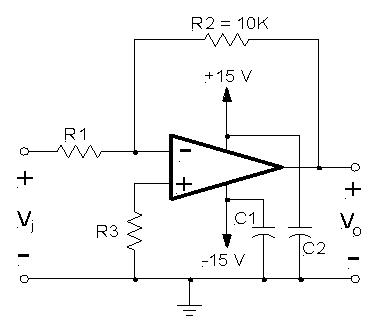
\includegraphics[]{img/ckt_tested}
  \caption{Circuit being tested.  $C_1 = C_2 = \SI{1}{\micro\farad}$}
  \label{fig:circuit}
\end{figure}

\subsection*{Test Configuration}
\label{sec:test_config}

\begin{figure}[hbtp]
  \centering
  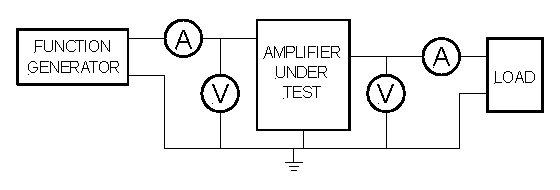
\includegraphics[]{img/test_config}
  \caption{\label{fig:test_config} Test Configuration}
\end{figure}

\section{Procedure}
\label{sec:procedure}

First, resistors $R_1$, $R_2$, and $R_3$ were measured with a
multimeter and recorded in Table~\ref{tab:table_01}.  Then the circuit
in Figure~\ref{fig:circuit} was constructed on a breadboard.  Next,
the configuration depicted in Figure~\ref{fig:test_config} was assembled.

Two Fluke multimeters served as the ammeters, and two input channels
of an oscilloscope served as voltmeters.  The function generator was
set to produce a sine wave with amplitude of
\SI{200}{\milli\volt_{rms}} @ \SI{1}{\kilo\hertz}, serving as the
voltage source, and a decade box set to \SI{200}{\ohm} serving as the
load.

With the load disconnected, the input voltage ($V_i$), input current
($I_i$), output voltage ($V_o$), and output current ($I_i$) were
measured and recorded in Table~\ref{tab:table_02}.  This step was then
repeated with the load connected.  Using these values with the
equations derived from the four amplifier models, measured values were
determined where direct measurement was difficult.

\section{Results}
\label{sec:results}

\begin{table}[hbtp]
  \centering
  \begin{tabular}{*{4}{c}}
    \textbf{Name} & \textbf{Nominal} & \textbf{Measured} & \textbf{\% Error} \\
    & (\si{\kilo\ohm}) & (\si{\kilo\ohm}) & \\
    \hline
    $R_1$ & 1 & 0.986 & 1.40 \\
    $R_2$ & 10 & 9.88 & 1.20 \\
    $R_3$ & 1 & 0.983 & 1.70 \\
  \end{tabular}
  \caption{Comparison of labelled and actual resistance.}
  \label{tab:table_01}
  \end{table}

\begin{table}[hbtp]
  \centering
  \begin{tabular}{*{5}{c}}
    & \multicolumn{2}{c}{\textbf{Voltage}} & \multicolumn{2}{c}{\textbf{Current}} \\
    & $V_i$ & $V_o$ & $I_i$ & $I_o$ \\
    & (\si{\milli\volt_{rms}}) & (\si{\volt_{rms}}) & (\si{\milli\ampere_{rms}}) & (\si{\milli\ampere_{rms}}) \\
    \hline
    \textbf{No Load} & 200 & 1.98 & 0.2 & nil \\
    \textbf{Load} & 200 & 1.98 & 0.2 & 9.52 \\
  \end{tabular}
  \caption{Comparison of electrical characteristics of the amplifier under load.}
  \label{tab:table_02}
\end{table}

\begin{table}[hbtp]
  \centering
  \begin{tabular}{l*{5}{c}}
    & \multicolumn{3}{c}{\textbf{Load}} & \multicolumn{2}{c}{\textbf{No Load}} \\
    & \textbf{Nominal} & \textbf{Measured} & \textbf{\% Error} & \textbf{Nominal} & \textbf{Measured} \\
    \hline
    $R_o$ (\si{\ohm}) & 0 & 0 & nil & 0 & 0 \\
    $R_i$ (\si{\kilo\ohm}) & 1 & 1 & 0.00\% & 1 & 1 \\
    $A_v$ & 10 & 9.9 & 1.00\% & 10 & 9.9 \\
    $A_i$ & 50 & 47.6 & 4.80\% & nil & nil \\
    $G_m$ (\si{\siemens}) & $\infty$ & $\infty$ & nil & $\infty$ & $\infty$ \\
    $R_m$ (\si{\kilo\ohm}) & 10 & 9.9 & 1.00\% & 10 & 9.90 \\
  \end{tabular}
  \caption{Comparison of values determined from amplifier models in Figure~\ref{fig:amp_models}}
  \label{tab:table_03}
\end{table}

\section{Conclusion}
\label{sec:conclusion}

As shown in Table~\ref{tab:table_03}, the amplifier models do closely
represent the amplifier used in the experiment.  The greatest
difference occurred in the current gain ($A_i$), largely due to $R_o$
being nearly zero.  This also causes $G_m$ to be very large.

\section{Appendix}
\label{sec:appendix}

\begin{figure}[hbtp]
  \centering
  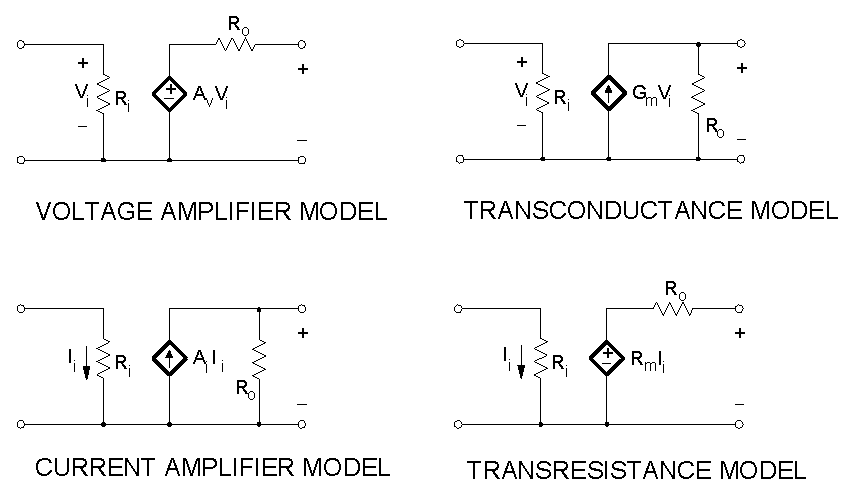
\includegraphics[width=\textwidth]{img/amp_models}
  \caption{\label{fig:amp_models} Four equivalent models of an amplifier}
\end{figure}

\subsection*{Equations}

% LaTeX sees blank lines as a start of another paragraph.  To avoid
% unnecessary vertical spaces between equations, and still visually
% separate in source, put a comment between them.
\begin{equation}
  \label{eqn:percent_error}
  \%_{error} = \frac{|measured - nominal|}{nominal} \times 100\%
\end{equation}
%
\begin{equation}
  \label{eqn:R_o}
  R_o = \frac{V_{noload} - V_{load}}{I_{load}}
\end{equation}
%
\begin{equation}
  \label{eqn:R_i}
  R_i = \frac{V_i}{I_i}
\end{equation}
%
\begin{equation}
  \label{eqn:A_v}
  A_v = \frac{V_o}{V_i}
\end{equation}
%
\begin{equation}
  \label{eqn:A_i}
  A_i = A_v \left(\frac{R_i}{R_o}\right)
\end{equation}
%
\begin{equation}
  \label{eqn:G_m}
  G_m = \frac{A_v}{R_o}
\end{equation}
%
\begin{equation}
  \label{eqn:R_m}
  R_m = A_v R_i
\end{equation}

\end{document}
